\documentclass[12pt]{article}
\usepackage{hyperref}
\usepackage{xurl}
\usepackage{graphicx}
\usepackage{xltabular}  % longtable + tabularx: wrapped columns that can break across pages
\usepackage{array}
\usepackage{xcolor}
\newcolumntype{Y}{>{\raggedright\arraybackslash}X}  % wrapped column, left-aligned

\usepackage[backend=biber, style=ieee]{biblatex}
\addbibresource{references.bib}


\begin{document}

% Title page
\pagenumbering{roman}
\begin{titlepage}
\begin{center}

% University logo and header
\vspace*{0.3cm}
\begin{figure}
    \centering
    
\includegraphics[width=0.15\linewidth]{uniandeslogo.png}
\end{figure}
\vspace{0.3cm}

{\Large\textbf{UNIVERSIDAD DE LOS ANDES}}
\vspace{0.5cm}

{\large\textbf{FACULTAD DE INGENIERÍA}}

\vspace{0.7cm}

{\normalsize Ingeniería de Sistemas y Computación}

\vspace{0.3cm}

{\normalsize }

\vspace{0.3cm}


% \vspace{3cm}

% Report title
{\LARGE\textbf{Undergraduate Thesis}}

\vspace{3cm}

% App name
{\Large\textbf{QuickR: A P2P Media Sharing Application}}
\vspace{0.3cm}

\vspace{1cm}

% Authors section
%\textbf{Submitted by:}

%\vspace{0.5cm}

{\textbf{Mateo López Cuartas}}

\vspace{4cm}


\vfill

% Date and university location
\today

\vspace{0.5cm}

{\normalsize Bogotá D.C., Colombia}

\end{center}
\end{titlepage}

\newpage
\tableofcontents

\newpage
\pagenumbering{arabic}
\setlength{\parindent}{20pt}

\section{Introduction}

\subsection{Context}
Ever since the turn of the millennium, the internet has had a significant impact on global communication technologies. By the year 2000, the internet was
already carrying 51\% of all information exchanged between any two-way communication networks, a figure that rose to 97\% by 2007~\cite{tech_capacity}.
This reliance on the internet has been steadily increasing over time, culminating in 2020 when quarantine and lockdown measures due to the pandemic 
made the internet an essential part of daily life for most people worldwide. This drastic change in people's lives led to an all-time high demand for 
applications that connect different individuals through digital means, such as Meta's Metaverse, the increased demand for virtual meeting software 
(Zoom, Google Meet, Microsoft Teams), and mass communication services like Discord and Slack.

It is in this context that the need to adapt these daily activities to a new digital environment arises; in this case, broadcasting and sharing multimedia 
content via streaming from one device (host) for others to view on their devices in real time, regardless of their geographical location.
Media streaming became popular through formal or academic means such as Zoom and Microsoft Teams, while the more casual media streaming needs were 
dominated by platforms like Twitch and Discord (the latter, although primarily used as a social messaging platform, also offers VoIP and video 
streaming services, which is the relevant service for this paper). The rapid expansion of video traffic on the internet, coupled with the staggering amount
of users of these services, has created a strong need to develop robust protocols that work quickly and efficiently under any type of connectivity conditions, as well 
as infrastructures that are sufficiently robust and scalable to meet the demand for these transmissions. 

This could be seen as a motivation by companies to restrict in certain ways some functionalities and features offered by these streaming services in a way that is 
actually profitable. Paywalls and subscription models are some of the most common ways companies and services implement a restriction that solves multiple problems at the
same time: first of all, it limits the number of users that can use the service at any given moment, which reduces maintenance costs and bandwidth usage; second, it produces
a source of income for the service provider, which can be used to improve the service and infrastructure; and third, it helps create a sense of exclusivity to the paying user. 
Some services that include these kinds of subscriptions are Discord, Google Meet, and Zoom. In the case of Discord, the service offers a subscription called Nitro that, besides
other benefits, allows the user to upgrade the stream quality from the free tier cap of 720p at 30fps to a maximum of 4K at 60fps, with a monthly cost of \$9.99 USD (as of November 2026). With Google Meet, 
the free tier besides allowing a call for only up to 60 minutes, hard limits the stream quality to 720p x 30fps, while any of Google's subscriptions allows for a maximum of 1080p x 30fps. Zoom, on the other hand, 
does not really restrict the stream quality, allowing content to be shared in the native resolution at 30fps for no extra cost, but it does recommend downscaling to 1080p to save on bandwidth. It also limits the free 
tier to 40 minutes per call, restricting the user not by the quality of the stream, but by the time they can use it.

Given the context of these service models with their constraints, it becomes apparent that users, even though there are multiple options for meeting their streaming needs, are still limited by the restrictions imposed
by these companies. Open source projects are alternatives to these services, but even though they can be more beneficial than closed-source by improving security, allowing way more flexibility, and fostering
community involvement by having collaborative development~\cite{open_source_benefits}, there are many cases in which these alternatives are not as widespread and used as the commercial ones. This lower popularity directly reduces the appeal to the 
common user to move onto these alternatives. Regardless, there exist a myriad of open source projects that act as cornerstones of the modern internet and computing as a whole, some of the main examples include the Linux kernel, the Apache web server, MySQL, and PHP.  And even outside of the scope of giant corporations running open source, even more projects exist that are maintained by small teams or even individuals.
There are many cases of these projects existing without an explicit commercial or financial interest, but rather as a means to solve a specific need, desire or problem someone encountered. Hausberg and Spaeth~\cite{hausberg2020open} on their analysis comparing Open Source Software (OSS) versus Open Source Hardware (OSH), state how
motivations behind OSS contributions stem from the individual's desire to contribute towards innovation that becomes a common good. It can be seen as the rational choice to provide a contribution for free, as the result afterwards becomes
a private, ongoing benefit. It is through this reasoning that one may explain the reasoning behind these projects taking off and staying relevant, even in the face of competition from commercial alternatives.

\subsection{Proposed Work: QuickR}
On account of the previous context, the proposed project is an open-source, Windows-specific desktop application that allows for screen sharing / video streaming between clients. This app is called QuickR and it distinguishes itself from other similar products on the market by 
combining the following characteristics into one desktop app:

\begin{itemize}
    \item No servers in between clients
    \item No need for an account nor subscription models
    \item No third parties relay nor store the stream
    \item No time limit
    \item Video quality determined by client's hardware and network conditions
\end{itemize}

These attributes allow the proposed application to stand out amongst the current market of remote desktop / live streaming / screen sharing options. It is published and free to use under the MIT License.

\subsection{Motivation}

Due to the large amount of corporate-maintained software on many everyday technological aspects, there has always been an interest on open source software development and maintenance. The democratization of software  
presents a unique opportunity for developers to create tailor-made solutions to their own problems or needs, benefitting from having a community of developers and users that can contribute to the project either by providing feedback, reporting bugs, contributing code, or by financially
backing the project. Besides, the characteristic of it being a private or open source project, developing a streaming service application involves a considerable amount of technical knowledge and integration in order to provide a robust and efficient
alternative for the user. Since it involves concepts of networking, video and audio encoding, synchronization, and UI/UX design, working on a streaming service application is a great way to learn by creating something tangible and useful, while also allowing a community of users to both
support and benefit from it. Another motivation stems from more personal reasons, as the interest in serverless alternatives where users have full control, coupled with the desire to watch movies with people who are geographically far away made way for this project idea to be born. 



\subsection{Objectives}
For this project, there will be a single main objective and a set of secondary objectives: 
\subsubsection{Main Objective}
The main objective is to design and develop a \textbf{Windows}-specific desktop application that implements a video streaming protocol that allows users to share real-time video and audio between devices from scratch.
\subsubsection{Secondary Objectives}
The secondary or auxiliary objectives are the following:
\begin{itemize}
    \item Develop a Peer-to-Peer (P2P) architecture that allows users to communicate between each other's devices.
    \item Implement a full transmission pipeline over UDP that allows for a \textbf{loss-tolerant} packet transmission.
    \item Build a user interface that shows received video and audio streams in real time.
    \item Compare the performance between existing alternatives (Google Meet, Microsoft Teams, Discord and Parsec) streaming tools and the developed application with measurable metrics such as end-to-end latency, framerate, bitrate, and CPU usage.
    \item For RTP-based services, compare the developed application in regards to packet loss and freeze percentage metrics. 
\end{itemize}

\subsection{Scope and Limitations}

For this project, the proposed application is limited to only work on Windows 10 and Windows 11 devices, as it uses specific API calls to these Operating Systems. Besides from this, it is not designed to allow more than 2 people to be on the same streaming session, as there is only one
broadcaster and one receiver. Encryption was not a consideration taken for the criteria of completing this project, as well as using a TURN server to help either by acting as a relay or a way to circunvent symmetric servers. This last characteristic also has a consequence of needing a separate 
medium to share each peer's connection code (the peer's IP address +  port tuple encoded into a string of uppercase letters and numbers. For example: BA1F3871:df4a). 

\subsection{Document Structure}
To detail the entire history, achievements and results of the project, first goes a section of definitions and background knowledge that will elaborate on necessary concepts. After that, it does a review of the state-of-the-art streaming tools and protocols, exploring the solutions that are already 
on the market. Subsequently, the next step will be the detail on the methodology taken for the design and implementation of the
application, to be followed by a series of tests and performance comparisons against the existing alternatives using packet analysis tools such as Wireshark.  


\section{Theoretical Background}
\begin{itemize}
    \item \textbf{Live Streaming:} The process of transmitting and/or receiving media content over the internet in real time and in a continuous manner.
    \item \textbf{Open Source Program:} Software and its source code for which it is publicly available to view, use, distribute, and modify mostly without restriction. Uses Licenses to establish any type of limitations and freedoms in regards to its use and distribution.
    \item \textbf{Closed Source Program:} Software whose source code is either partially or fully restricted from public access, which is usually developed and maintained by a private company or organization.
    \item \textbf{Peer-to-Peer (P2P):} Type of network architecture in which every device (called peer or node) connects and shares resources without any centralized server. Every node inside of this network can be a consumer and/or provider of resources.
    \item \textbf{Network Address Translation (NAT):} A networking service that maps private IP addresses to a public address for communication outside the local network.
    \item \textbf{NAT Hole Punching:} Technique used to establish P2P connections in different networks. This technique works by having both nodes send a "dummy" packet to each other, thus opening a "hole" in the Firewall to that specific address. Any further packet from that address will be treated as a reply to the initial "dummy" packet and will be allowed through into the network.
    \item \textbf{Full Cone NAT:} Defined under RFC 4787 as \textit{Endpoint-Independent Mapping}, Full Cone is a NAT service that maps an internal IP address and port to a single, static external IP address and port, allowing any external host on the internet to send packets to that external address and reach the internal device. This mapping is extremely permissive and maximizes compatibility for peer-to-peer applications at the expense of lower inbound security.
    \item \textbf{Symmetric NAT:} Defined under RFC 4787 as \textit{Address and Port-Dependent Mapping}, Symmetric NAT is a NAT service that maps a distinct external port to each outgoing IP and port tuple. Since the external port mapping varies depending on each destination, this service prevents 
    incoming traffic from external devices and thus turns Hole Punching useless.
    \item \textbf{Session Traversal Utilities for NAT (STUN) servers:} Types of publicly accessible servers that allows devices living on private local networks to discover their public IP address and port number. When a device sends a request to one of these servers, the NAT modifies the packet header with the router's public IP and address, and the server sends a reply packet with that exact information as the answer. 
    These servers are pivotal for P2P communications, but don't work for devices on a private network with a Symmetric NAT configuration.  
    \item \textbf{Traversal Using Relays around NAT (TURN) server}: Types of publicly accessible servers that act as relays between P2P devices when the network restricts direct communication (most common case being Symmetric NAT). These servers should guarantee that they do not interfere with nor record any of the transmitted passages.
    \item \textbf{Latency:} Streaming-based metric that measures the time delay between a piece of data (a frame) getting captured and the moment it arrives at the destination. In this case, it will be measured by comparing packets with the same sequence header by computing the difference between their timestamps.
    \item \textbf{Frames Per Second (FPS):} Amount of distinct images (frames) the client screen can display, measured per second.
    \item \textbf{Codec:} Process that can compress video into a smaller size and can afterwards decompress it using mathematical algorithms. Some common codecs that are mentioned in this document are H.264, H.265, VP9, AV1, among others.  
    \item \textbf{KeyFrame:} In a codec-compressed video, KeyFrames are complete frames that store all of the frame's data by itself without a reference to any other frames. 
    \item \textbf{DeltaFrame:} In a codec-compressed video, DeltaFrames are a type of frame that only contains the information of changes in regards to the previous frame. These frames are in most cases smaller than KeyFrames, but depend on the decoder having the exact previous frame as a reference to work properly.
\end{itemize}

\section{State of the Art}
    \subsection{Parsec} Parsec is a desktop application whose main goal is to allow for a seamless experience using remote desktop connections, with online gaming as the primary focus, but allowing for connections to cloud devices and personal computers as well.
        According to the information provided by the official Parsec Team (including 2 different blog posts and a talk at Code Driven NYC~\cite{parsec_streaming,parsec_udp_primer,parsec_udp_slides}), this application's streaming logic was built based these
        priorities in the following order of importance: \textbf{latency, then frame rate, then video quality}. To achieve the goal set on reducing latency to the absolute minimum, many standard technologies were
        tested, starting with both UDP and TCP protocols. The developers took both protocols and decided which attributes were desirable to bring over to a new, proprietary protocol that met all of the needs necessary for Parsec to provide a seamless video game streaming experience:
        
        \textbf{TCP:} 
            \begin{enumerate}
                \item Reliability and reordering.
                \item Stream Semantics
                \item ACK to confirm packet reception 
            \end{enumerate}
        
        \textbf{UDP:} 
            \begin{enumerate}
                \item Stateless hole-punching
                \item Connection state and handshake via DTLS
            \end{enumerate}
        Due to the necessity of bringing some (but not all) characteristics of each protocol, the Parsec team developed their own protocol called BUD (Better User Datagrams) for their service. This protocol works by diverging from the standard
        TCP behavior of working in any network condition
        by throttling the performance to give priority to the correct delivery of the packets. Instead, it assumes the user has more bandwidth than a tested minimum (not a concrete value, but according to the Code Driven NYC talk, it is $\sim30$ Mbps with less than a 50ms RTT).
        By using this assumption, the algorithm does not have to concern itself with cases of poor connection but rather works with known stable connections. 
        
        The most important characteristics regarding the BUD protocol are the following:
        \begin{itemize}
            \item NAT traversal by hole punching: To bypass firewalls blocking incoming requests by the incoming device, the protocol uses a staple technique based on UDP's nature to establish direct Peer to Peer connection.
            \item Congestion control not done via internal packet sending limits, but instead via the encoder. Using H.264 as the main video encoder, Parsec controls its bitrate frequently depending on the network congestion and RTT (Round-Trip Time). 
            By varying the bitrate, the algorithm can reduce load on the bandwidth without halting packet sending, so that the client can still receive data and show live updates on the screen without any added latency. 
            \item Fast packet retransmission: By having ACK packets and a buffer that loads packets and updates them at runtime (which is another benefit of never having to reallocate memory), the algorithm can notice quickly if a packet $N$ hasn't received an ACK while packet $N+1$ already received
            its own ACK. When this happens, it triggers a quick retransmission of packet $N$ to avoid any delays. There is also a slow retransmission as a failsafe.
            \item A very concise and small packet header with Sequence Number, Data Type and Payload.
        \end{itemize}
        With these characteristics, BUD is able to perform with an exceptional quality in various environments. During live showcases, Parsec was able to perform at near 30 fps with packet loss between 5 and 10\%. Nonetheless, the documents state the software still falls behind on
        symmetric NATs (they restrict the hole punching method needed for the first connection establishment), degraded networks are still not contemplated for the algorithm's performance, and creating a protocol with custom tools brings a great deal of technical debt and issues that have to be
        solved in-house.  

        \textbf{How it compares to QuickR:} Similar to QuickR, the BUD protocol was developed after realizing that using either TCP or UDP by themselves as a transport medium for quickly-changing data such as video streams will not be enough. It also uses hole punching similarly to how QuickR does to establish connections.
        However, Parsec has many differences in its design logic and architecture, such as congestion control via a variable bitrate at runtime, a 'ring' buffer where frame data is allocated and overwritten by new frames to avoid memory reallocation, and end-to-end packet encryption.  
    \subsection{Discord} 
    Although the Discord Application offers a myriad of services, mainly focused on instant messaging and VoIP communications, it also includes a feature called \textit{Go Live}, which is the company's feature for screen sharing inside of the app's voice channel. 
    According to the blog detailing this service's inner workings, \textit{Go Live} works with a pipeline that relies on three different but interconnected components: \textbf{Screen capture, data encoding, and transport.}~\cite{discord_streaming}
    \begin{enumerate}
        \item \textbf{Capture:} For capture to go as smooth as possible, the algorithm checks available capture methods the device's operating system provides, and picks the best one available at the moment. If that capture method fails, the system falls back 
        into the next best alternative to keep the stream going without any issues. Some of the mentioned methods include the OS's own APIs, or injecting a DLL into the game to read what the screen renders and sending it directly to the pipeline. For the audio component, 
        the app captures the audio of the window that was selected for sharing, but no audio is sent if the entire device's screen gets selected. No definite reasoning is provided for this, but a reasonable explanation would be that, since the main goal of screen sharing is to be used
        inside of VoIP calls, sharing the entire device's audio would probably mirror the other participants' voice audio, worsening the experience for the clients that are watching the screen stream. 
        \item \textbf{Encoding:} Since a single \textbf{uncompressed} 1080p frame can be as large as 6MB, an encoder is completely necessary to avoid bottlenecking the network socket and to allow frames to be sent at a faster rate. Every time a \textit{Go Live} session is initiated, all clients negotiate a
        codec that can be used to decode the packets by every participant of the call. The algorithm prioritizes hardware encoders (from GPUs) over software encoders whenever possible to attempt to reduce CPU load. The more commonly available codecs are VP8 and H.264, with HEVC and
        AV1 being available on some devices. When the network quality degrades, the algorithm drops frames to relieve congestion until it improves.  
        \item  \textbf{Data Transmission: } Unlike Parsec's system, \textit{Go Live} is not Peer-to-Peer. Instead, it relies on Discord's own media relay servers to get each participant's IP address and relaying the data packets to the correct recipients at all points of the process. This is primarily done
        due to privacy purposes, as users do not get access to others' private information even if they are on the same call. This transport is built over WebRTC with video and audio packets being sent separately. The sending rate is dynamically capped by the user with the slowest network, so everyone gets 
        the same experience.
    \end{enumerate}
    When the receiver gets the video and audio packets, the client synchronizes both of these streams on the client device before showing it to the user. A known issue based on the technical decisions taken for this approach is that the VoIP audio and the stream are not synchronized, as they are managed by 
    different systems. This puts pressure on the developers to reduce stream latency as much as possible to avoid degrading the users' experience with the service.

    \textbf{How it compares to QuickR:}  \colorbox{red!50}{TODO}

    \subsection{RustDesk}
    RustDesk~\cite{rustdesk_repo} is an open-source alternative to TeamViewer, providing remote desktop services. It is written in Rust, and it falls under the AGPL-3.0 License. Even though Rustdesk offers a remote desktop service instead of a strict video-streaming one, both services work under similar logic and architectures. 
    The main characteristics of to be taken into consideration for this project are the following:
    \begin{enumerate}
        \item \textbf{Initial connection and TURN by the hbbs/hbbr servers:} Rustdesk provides a lightweight server called hbbs that holds IP and port information between devices that are attempting to connect, and coordinates the hole punching process to get a connection. If that process fails (for example, due to Symmetric NAT configurations), 
        there is another server called hbbr that can act as a TURN server and relay messages between nodes.~\cite{rustdesk_server}
        \item \textbf{Video and audio codecs:} Utilizes VP8,VP9, and AV1 software codecs for video compression and Opus for audio compression. It is stated to also have H.264/H.265 as hardware encoders as a fallback.
        \item\textbf{End-to-end encryption:} Uses the NaCl library to provide end-to-end encryption not even the hbbs can access or tamper with during remote desktop sessions. Both nodes also use asymmetric encryption to check the authenticity of the hbbs server on connection start, using an Ed25519 key-pair. 
    \end{enumerate}

    \textbf{How it compares to QuickR:} Being an open-source, Rust-based real-time video streaming service, this is the closest resemblance to QuickR. As such, it presents a great amount of similarities in the architecture and design choices, but it also has some characteristics that QuickR lacks, such as a workaround to
    Symmetric NATs (the TURN server on hbbr), automatic peer discovery via ID, and end-to-end encryption. Unfortunately, this incurs into some drawbacks as the trade-off for some of the advantages, such as needing an intermediary server for any and all communications (either for hole punching or for packet relay).
    Also, it is important to note that since RustDesk is a remote desktop control service, it includes many other microservices necessary to fulfill that need, such as a more specialized UI, coupled with controller input detection logic (mouse movements, keyboard presses) that QuickR does not need to replicate or find an alternative for.   
    
    \subsection{WebRTC}
    Although WebRTC is not a program nor app, it is a protocol standard, as defined by RFC 8825~\cite{rfc8825}, plus around 20 other RFCs that document many of its characteristics. This protocol is tailored for needs such as direct P2P audio and video transmission inside of desktop, web, and mobile apps natively. Some of its most important 
    characteristics are:
    \begin{itemize}
        \item Allows for both STUN and TURN-based server use to establish and maintain connection between peers.
        \item Mandatory encryption using DTLS-SRTP to generate symmetric keys and secure channels afterwards. Media gets sent over SRTP (Secure Real-time Transport Protocol).
        \item Uses VP8 and H.264 for video codec, while using Opus and G.711 for audio codecs.
        \item Advanced congestion control based on adjusting the encoder's bitrate to allow for a smoother transmission. This process is triggered by metrics such as delay changes via RTT and packet loss rates
        \item Loss recovery by fast retransmissions based on the reception of NACKs (message indicating the packet was \textbf{not} received correctly). Forward error correction is also used for this standard, as it allows to use the extra parity bits to fix errors on received packets without needing a retransmission.
        \item Audio / Video synchronization using Sender Report timestamps, which triggers jitter buffers to allow any of the 2 mediums to catch up to the other one.
        \item Able to be used for a pure P2P service, but also extendible to have different types of servers in between nodes.
        \item KeyFrame requests are sent via PLI (Picture Loss Indication) requests. When the decoder notices a critical error with the decoding or necessary frame context is missing, the receiver can send a PLI which forces the sender to send a fresh KeyFrame as soon as possible.
    \end{itemize}

    \textbf{How it compares to QuickR:} In contrast to QuickR, the WebRTC standard is extremely mature, has been audited, and in general purposes fulfills all requirements needed for QuickR to work, and even offers solutions for problems QuickR has yet to fix and/or implement. However, it is not used for this project because of these same reasons.
    As a fully developed standard with a myriad of tested implementations on any framework or language (including a fully complete WebRTC implementation in Rust), all of these are very complex and contain many more services not needed for the requirements stated previously for the proposed app. Besides, using these already developed solutions obfuscates
    many networking concepts, as they are already solved and taken into account. By working on developing a new protocol to fit the exact needs stated beforehand, the user has much more control over every layer of the networking stack plus every step of the streaming process. For this reason, this project prioritizes the learning process of building
    a whole protocol with basic tools rather than having a solution that can solve all of the shortcomings of QuickR at the cost of limiting the learning experience building the app gives. 

    \subsection{General comparison}
    Taking into account the alternatives described above, Table~\ref{tab:comparison} summarizes the main architectural and design choices/attributes of each one, alongside those of QuickR.

   \begingroup
    \footnotesize
    \renewcommand{\arraystretch}{1.3} 
    \setlength{\tabcolsep}{4pt}
        \begin{xltabular}{\textwidth}{|>{\raggedright\arraybackslash\bfseries}p{2.4cm}|Y|Y|Y|Y|Y|}
            \caption{Comparison between the reviewed alternatives and QuickR.}
            \label{tab:comparison}\\
            \hline
            & \textbf{Parsec} & \textbf{Discord (\textit{Go Live})} & \textbf{RustDesk} & \textbf{WebRTC} & \textbf{QuickR} \\
            \hline
            \endfirsthead
            % --- header repeated on each following page ---
            \multicolumn{6}{l}{\textit{Table~\thetable\ (continued)}} \\
            \hline
            & \textbf{Parsec} & \textbf{Discord (\textit{Go Live})} & \textbf{RustDesk} & \textbf{WebRTC} & \textbf{QuickR} \\
            \hline
            \endhead
            % --- footer at the bottom of pages that continue ---
            \multicolumn{6}{r}{\textit{Continued on next page}} \\
            \endfoot
            % --- footer of the last page (empty) ---
            \endlastfoot

            Type
                & Proprietary app
                & Proprietary app
                & Open-source app
                & Protocol standard
                & Open-source app \\
            \hline
            Architecture
                & Direct P2P
                & Client--server (media relayed by Discord's servers)
                & Direct P2P first, relay as fallback
                & P2P, or through servers depending on the deployment
                & Direct P2P only \\
            \hline
            NAT traversal
                & UDP hole punching
                & Not needed (clients connect to servers)
                & UDP hole punching coordinated by hbbs
                & ICE with STUN
                & STUN + UDP hole punching \\
            \hline
            Relay fallback
                & No
                & Always relayed
                & Yes (hbbr)
                & Yes (TURN)
                & No \\
            \hline
            Transport
                & BUD (custom, over UDP)
                & WebRTC (RTP over UDP)
                & Custom (over UDP/TCP)
                & RTP/RTCP over UDP
                & Custom RTP-inspired protocol over UDP \\
            \hline
            Encryption
                & DTLS
                & Yes (DAVE protocol~\cite{discord_DAVE})
                & End-to-end (NaCl)
                & Mandatory DTLS-SRTP
                & None (future work) \\
            \hline
            Video / audio codecs
                & H.264 / No documentation on audio codecs
                & VP8, H.264, HEVC, AV1 / Opus
                & VP8, VP9, AV1, H.264, H.265 / Opus
                & VP8, H.264 / Opus, G.711
                & H.264 (OpenH264) / Opus \\
            \hline
            Congestion control
                & Encoder bitrate adapted to RTT and congestion
                & Rate capped by slowest viewer; frame dropping
                & Adaptive quality
                & Delay- and loss-based (GCC)
                & Fixed bitrate cap \\
            \hline
            Loss recovery
                & Fast and slow retransmission (ACK-based)
                & Inherited from WebRTC
                & --
                & NACK + retransmission, FEC, keyframe requests
                & Keyframe (IDR) requests \\
            \hline
            Open source
                & No
                & No
                & Yes (AGPL-3.0)
                & Yes (e.g.\ libwebrtc, webrtc-rs)
                & Yes (MIT) \\
            \hline
            Servers required
                & Yes (account and connection brokering)
                & Yes (always)
                & Yes (hbbs, self-hostable)
                & Signaling server (+ TURN/SFU if used)
                & Public STUN server only \\
            \hline
        \end{xltabular}
    \endgroup

Given the comparison with other modern solutions to the same problem, some similar answers to specific problems are obvious: all processes rely on UDP as a base to start the packet transfer, even if it is later improved by any of multiple additions (BUD, fast retransmissions, etc.). 
Similarly, it is evident how all native P2P systems use hole punching to establish connections, plus using Opus as the preferred codec for all solutions that state their audio codec. Another solution to a very important problem, although not stated to be used by all systems, is the KeyFrame request. 
Although only WebRTC explicitly describes using it, having logic determining how to ask for a keyframe when the decoder cannot decode any more for any reason is a sound answer to stream degradation due to the nature of UDP. All of these characteristics are shared with the proposed QuickR software.

Besides similarities with QuickR, there are some details of attributes other applications implement but QuickR lacks, for example, symmetric NAT solutions, streamlined peer connection, and reactiveness to network congestion. Unfortunately, all of these are characteristics that demand at the very least
dedicated servers to aid the clients. This incurs into a heavier need for more robust infrastructure and external services, which goes against QuickR's goals. Although it complicates some of the elements of the app, having a functioning media streaming application that guarantees being open source, not
needing an account nor other servers (excluding the public STUN server) cements the niche QuickR is trying to fill.

Having the design choice of excluding external helper servers from the scope of the project certainly puts QuickR at a disadvantage against the already working services explained before, especially since it lacks providing a relay fallback, bypassing symmetric NAT, having dedicated packet encryption, and congestion control.
Nonetheless, these are deliberate limitations to the scope of the current project, and would be addressed in future work. The performance evaluation at Section~\ref{sec:results} shows the impact of having a minimal design in comparison to the alternatives. 

\section{Methodology}

\colorbox{red!50}{TODO}

\section{QuickR: Design and Implementation}

QuickR is an application built entirely on the Rust programming language, using to its advantage the compiled nature of this language. This application has 3 interconnected core components whose functionalities interweave between each other to achieve the result of showcasing a real time stream: 
\textbf{the Transport Protocol, the Screen/Audio Capture Logic, and the Graphical User Interface. } The following subsections delves into the details for each one of these main components.

\subsection{Architectural Overview}
Figure~\ref{fig:architecture} shows a general outline of the main components of the process and the steps QuickR takes to perform its objective. It is important to note how there are no external steps, intermediaries or processes outside of the two peers exchanging information between each other. That is, excluding the
single-time-use STUN server that gives each peer its own public facing IP address + port tuple, and the external communication medium used between both peers to exchange their connection codes. Further routines each peer executes are detailed on the following chapters.
\begin{figure}[htbp]
    \centering
    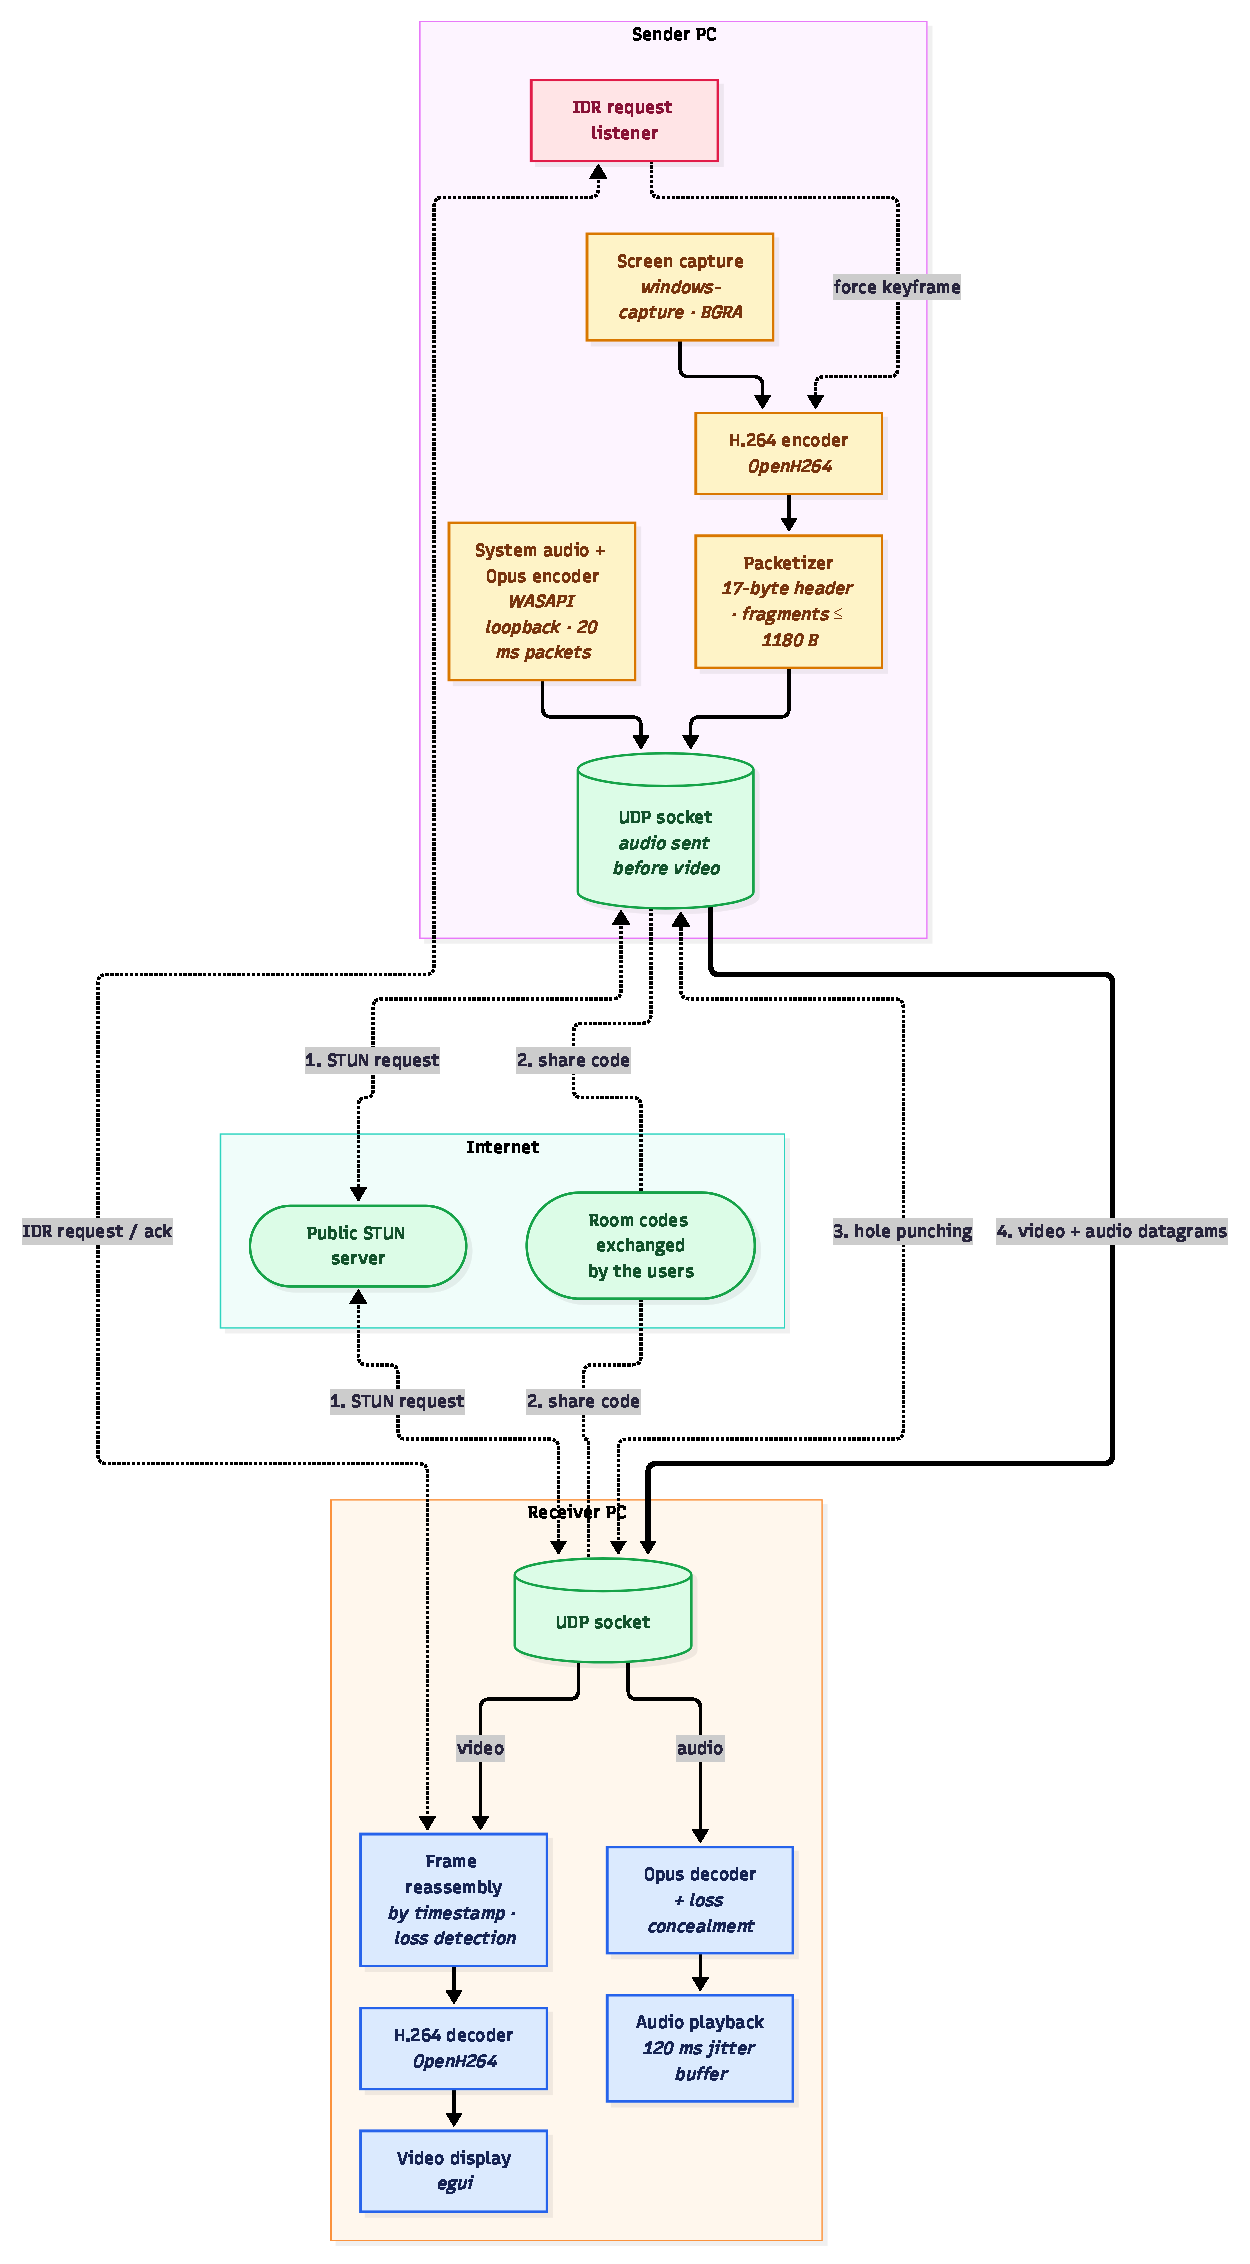
\includegraphics[height=0.75\textheight]{architecture2.pdf}
    \caption{Overview of QuickR's architecture. Numbers indicate the steps taken to establish connection and send stream packets.}
    \label{fig:architecture}
\end{figure}

\newpage
Figure~\ref{fig:header} details another relevant aspect of the program's own datagram architecture, which is its custom header structure. It is 17 bytes long and every packet shared between the 2 peers uses it. Following is the detail and reasoning behind every attribute's inclusion in the header:

\begin{figure}[htbp]
    \centering
    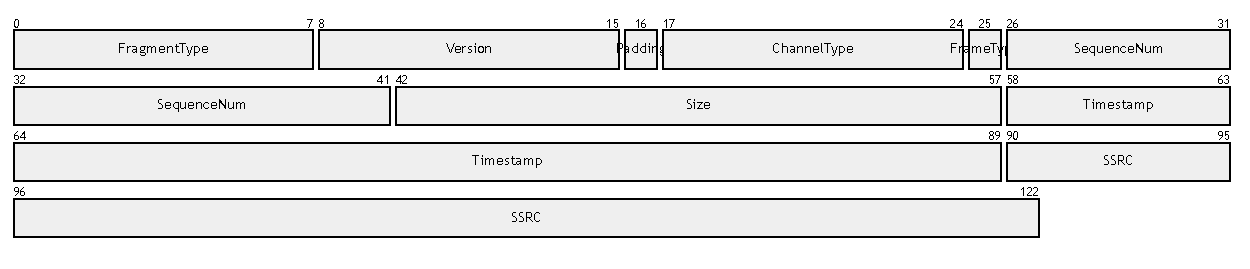
\includegraphics[width=\textwidth]{header1.pdf}
    \caption{QuickR's custom packet header}
    \label{fig:header}
\end{figure}

\begin{itemize}
    \item FragmentType (1 byte): A u8 integer between 1 and 4 that states if the packet is a fragment of a larger structure or if the whole structure is contained inside of the 1200 byte payload. If the structure has to be fragmented, (in most cases, a large frame that cannot be sent in one single payload), it will detail if the payload is
    the start of the structure (1), the end (3), or any fragment in between (2). If the structure can be sent without fragmentation, it will be marked as Unfragmented (4).
    \item Version (1 byte): A u8 number indicating the protocol's version. Fixed at 1 for the moment, but implemented to be updated in the future.
    \item Padding (1 bit): A bool determining if the payload has padding at the end. Unused for now, but designed with code extensibility in mind
    \item ChannelType (1 byte):  A u8 integer between 1 and 5, the receiver can use it to determine what to do with the packet as follows:
    \begin{enumerate}
        \item Video: The packet contains video information of a frame.
        \item Audio: The packet contains 200ms of audio.
        \item \begin{sloppypar}
                   Control: Generic type for control messages in regards to the stream. For example, it can be used to request a different resolution to be sent from that point onwards, or a request for a new IDR when the decoder encounters an error with the current frame and needs a refresh.
               \end{sloppypar}
        \item Sync: Packets that contain the sync channel are part of the hole punching process detailed in ~\ref{sec:connection}
        \item IdrAck: ACK packet the receiver sends back to the broadcaster after it requested an IDR to prevent unnecessary IDR retries. Explained further on ~\ref{sec:screencap}
    \end{enumerate}
    \item SequenceNum: A u16 integer that determines the sequence number of the payload. Due to the nature of sending packets by UDP, there is no guarantee of an ordered arrival of payloads, so this allows the receiver to reorder arriving packets. This attribute is only relevant for packets with ChannelTypes 1 (video) or 2 (audio), and the value of sequencenum is 0 for any other case. 
    \item Size: A u16 integer that stores the size in bytes of the payload.
    \item Timestamp: A u32 integer that details the exact time in milliseconds the header was created. This is useful mostly for frame reconstruction, as every fragment of the same frame has the same timestamp value.
    \item ssrc: Based off of RFC 3550\cite{rfc3550}, the ssrc is a ID stored on a u32 integer that is unique for each peer's audio or video stream. Designed for a future implementation of QuickR when multiple peers can connect and stream at the same time to the same connection, this ID guarantees that video or audio packets from one peer are not mixed with another's packets. 
\end{itemize}   

\subsection{Connection Establishment}
\label{sec:connection}

For connection establishment, there are 4 main steps to successfully allow the two nodes/peers to send information between each other:
\begin{enumerate}
    \item STUN server request (on \colorbox{gray!20}{`/transprot/src/stuntry.rs`}): As soon as the program boots up, each peer sends a Binding Request (20-byte payload) to a hardcoded STUN server, in this case 'stun4.l.google.com:19302'. The server accepts the connection and the Binding Request and replies with a XOR Mapped Address. This address can be converted into the public IP Address + port tuple easily and loaded on local memory. 
    \item Public Address to connection code conversion (on \newline \colorbox{gray!20}{`/commons/src/ip\_converter.rs`}): After receiving the public address tuple from the STUN server, internally the program converts both the IP address and port into a string by transforming each octet into its Hexadecimal representation (for example, 192 would become C0) plus dropping the periods (.) in between octets. The same process is done with the 
    port number, but both address and port hexadecimal representations are separated by a colon. For example, if the original tuple is '186.155.19.201:29539', the connection code would be 'BA9B13C9:7363', which, although not the best compression method, does reduce character amount per code and makes it easier to share between peers. 
    \item Connection code sharing: This step generates some friction, as the current implementation of QuickR does not offer any in-app methods to share these connection codes between the two devices. It is necessary for both users to use a different medium to share these codes and register them on the app. 
    \item Hole Punching: Once both devices know each other's connection code, they revert it back to the IP address + port tuple, and send via UDP a packet containing only the header with ChannelType = 4, for a Sync Channel. These messages are sent 19 times with a delay of 400ms in between. This is because of the requirement of the other device to have already opened up the "hole" on their firewall so that the packet from the other peer gets delivered correctly, 
    thus the need for multiple packets. Once any device gets a single Sync packet from the other peer, they have guaranteed the hole punching worked and there is a way to communicate with the other device. To make sure the other device has also received at least 1 packet to confirm connection, it sends 5 more Sync packets in quick succession (delay reduced to 100ms in between packets) but it itself starts discarding any leftover incoming Sync packet. After both devices send the 5 packets each, they are both
    ready to start the transmission, and the receiver is ready to get packets with the Video and Audio ChannelTypes.
\end{enumerate}

Figure~\ref{fig:connseq} illustrates the step-by-step process of achieving the connection detailed above. 

\begin{figure}[htbp]
    \centering
    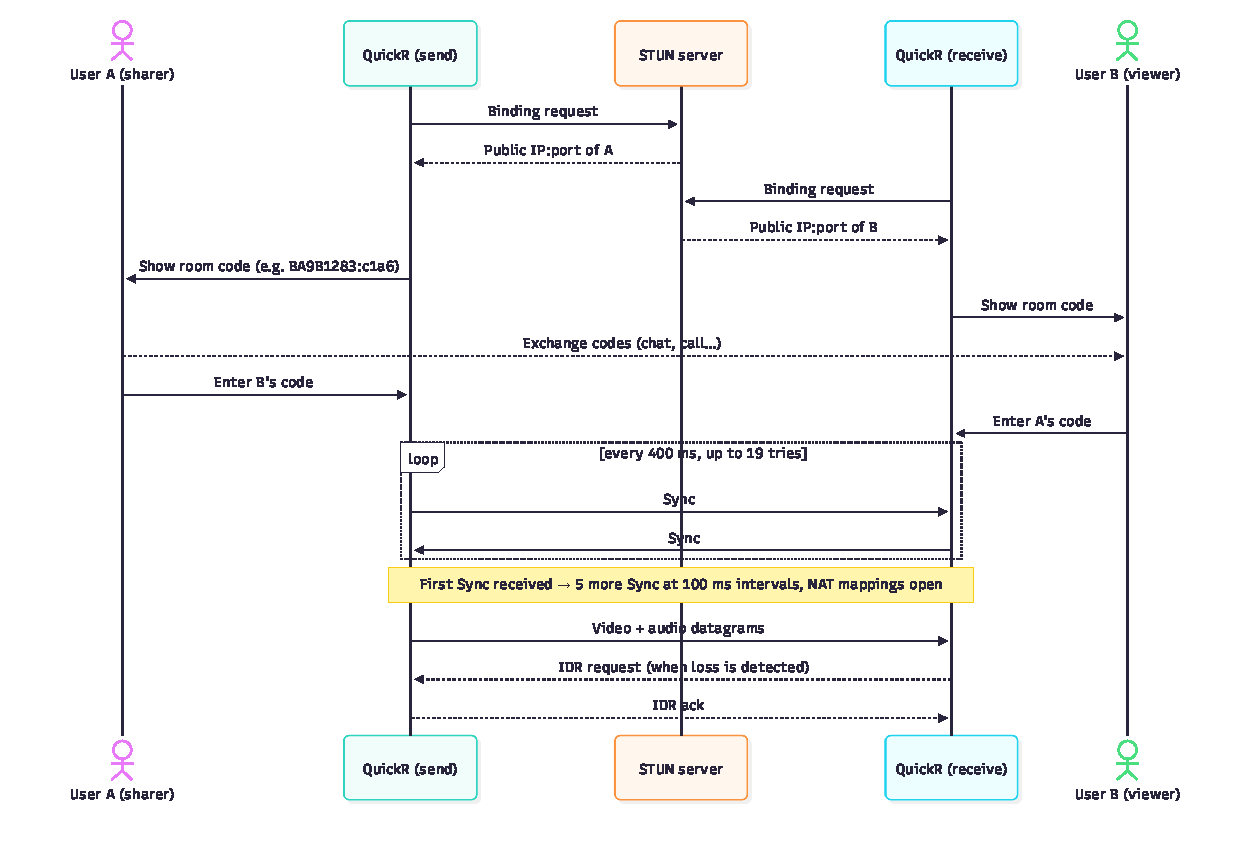
\includegraphics[width=\textwidth]{conn_seq1.pdf}
    \caption{QuickR's connection establishment sequence}
    \label{fig:connseq}
\end{figure}

\subsection{Transport Logic}


\subsection{Screen Capture Pipeline}
\label{sec:screencap}

\subsection{Audio}

\subsection{Graphical User Interface}

\subsection{Code Repository Structure}

\section{Results and Discussion}
\label{sec:results}

\subsection{Results}


\subsection{Conclusion}









\printbibliography
\end{document}